\documentclass[./thesis.tex]{subfiles}
\begin{document}
\chapter{Type theory}
\label{chap:type-theory}

Whatever the meaning of the Curry-Howard correspondence, its utility is
circumscribed by the fact that \IPL{}/\TLC{} as
presented do not match the expressive power of classical \FOL{}:
there are no types expressing quantification over some domain, nor propositions
or relations that may ``apply'' to terms and variables. Certainly, they are
missing the infinite structures of classical set theory.

The system described in this section enriches \TLC{} with
\textit{dependent types} (\cref{sec:dependent-types}) and a few more base types,
including our first examples of \textit{inductive types}
(\cref{subsec:natural-numbers-and-lists}). Additionally, we define and include
Voevodsky's univalence axiom (\cref{sec:univalence}). The
resulting system (univalent type theory, or \UTT{}) has similar
expressive power to \ZFC{}+\FOL{}.\footnote{Indeed, the
  ``set types'' (\cref{def:sets}) behave very much like sets in classical
  mathematics, especially when a few classically-minded axioms are assumed. See
  \cite{book} for more commentary.

  Conversely, \ZFC{} and infinitely many inaccessible cardinals models the
  similar system \HoTT{} (via Voevodsky's simplicial set construction).}

\UTT{} mirrors the type theory $\caH'$ of \cite{homotopy-limits}, which itself
is the system $\caH$ in \cite{inductive} and \cite{homotopy-initial} with the
addition of the natural numbers and universes. The results of
\cref{chap:coinductive-types-in-univalent-type-theory} don't
require the full power of homotopy type theory (\HoTT), specifically we leave
out the axioms asserting the existence of higher inductive types.

\begin{notation}
  Henceforth, we denote variables and meta-variables with the same
  script.
\end{notation}

\section{Dependent types}
\label{sec:dependent-types}

One of the slogans of dependently typed programming is that ``types are
terms''. Propositions, like proof terms, can now be subsumed as objects of study
in their own right.

\begin{definition}
	A \define{dependent type} or \define{type family} is a term with a free
  variable of a specified type, which, when filled in with any term of said
  type, is a type. In other words, $B$ is a dependent type with variable of type
  $A$ if for some $Γ$,
  \begin{equation*}
    Γ,a:A⊢\type{B}.
  \end{equation*}
  That is, a dependent type is a \textit{type} that \textit{depends} on a
  \textit{value}. 
\end{definition}

In the interpretation of types as propositions, dependent types correspond to
predicates. The following illustration uses several concepts yet to be
introduced, trust that it can be made precise after the next few sections.
Suppose we have a type $ℕ$ with introduction rules (or ``constructors'')
\begin{align*}
  \prftree[r]{}
    {}
    {Γ ⊢ 0:\ℕ} &&
  \prftree[r]{}
    {Γ ⊢ n:\ℕ}
    {Γ ⊢ \apply{\suc}{n}:\ℕ}
\end{align*}
($0$ is what a logician might call a ``non-logical constant'' and $\suc$ a
``function symbol''). We might define a type family
\begin{alignat*}{3}
  &\apply{\ttfun{Even}}{0} &&\defeq \unittype  \\
  &\apply{\ttfun{Even}}{(\apply{\suc}{0})} &&\defeq \emptytype  \\
  &\apply{\ttfun{Even}}{(\apply{\suc}{(\apply{\suc}{n})})} &&\defeq \apply{\ttfun{Even}}{n}
\end{alignat*}
Then $\apply{\ttfun{Even}}{n}$ is inhabited ($≅$true) when $n$ is even, and
empty ($≅$false) otherwise.

\begin{remark}\label[remark]{rmk:n-true}
	Here's an opportunity for confusion: is a type like $\ℕ$ ``true''? It's
  certainly inhabited. Again, we, as humans, must decide which types to
  interpret as propositions, properties, etc. \Cref{sec:h-levels}
  covers types that essentially contain no other information other than whether
  or not they are inhabited, these are called ``propositions''.
\end{remark}

\subsection{Π-types}
\label{subsec:pi-types}

The \define{dependent function type}, or Π-type, generalizes the direct product
and function types. It is formed via the following rule:
\begin{equation*}
  \prftree[r]{}
    {Γ ⊢ \type{A}}
    {Γ, a:A ⊢ \type{B}}
    {Γ ⊢ \type{\pitt{a:A}{\apply{B}{a}}}}
\end{equation*}
It is \textit{crucial} to remember that the Π (just like λ) scopes over the
entire rest of the expression, unless otherwise delineated by parentheses.
This type represents functions with output \textit{types} that depend on the
\textit{value} of an \textit{input}. They associate to each $a:A$ some element
of the type $\apply{B}{a}$. Thus, the introduction rule (dropping hypotheses
that appear in the formation rule):
\begin{equation*}
  \prftree[r]{}
    {Γ, a:A ⊢ b:\apply{B}{a}}
    {Γ ⊢ \λ{a}{b}:\pitt{a:A}{\apply{B}{a}}}
\end{equation*}
where the term $b$ usually has a free occurrence of $a$. If it doesn't, the Π-type
specializes to the normal function type. The elimination, computation, and
unicity rules are also straightforward generalizations of normal functions types:
\begin{gatherjot}
  \prftree[r]{}
    {Γ ⊢ {f}:\pitt{a:A}{\apply{B}{a}}}
    {Γ ⊢ {a}:{A}}
    {Γ ⊢ \apply{p}{a}:\apply{B}{a}}
  \qquad
  \prftree[r]{β}
    {Γ, a:A ⊢ b:\apply{B}{a}}
    {Γ ⊢ x:A}
    {Γ ⊢ \apply{\λ{a}{b}}{x}\jdeq b[a\defeq x]:\apply{B}{a}} \\
  \prftree[r]{η}
    {Γ ⊢ f : \pitt{a:A}{\apply{B}{a}}}
    {Γ ⊢ \λ{x}{\apply{f}{x}}\jdeq f:\pitt{a:A}{\apply{B}{a}}}
\end{gatherjot}

Under the types-as-propositions interpretation, Π-types correspond to universal
quantification. A term of type $\∏{a:A}{\apply{B}{a}}$ takes each $a:A$ to a
proof or witness that $B$ holds of $a$. Loads of examples to follow throughout.

\begin{example}
  The following example illustrates that dependent types truly allow for
  \textit{arbitrary expressions} to appear at the type level:
  \begin{gather*}
    f:\∏{t:A+B}{\apppply{\case}{(\λ{a}{\unittype})}{(\λ{b}{\unittype×\unittype})}{t}} \\
    f \defeq \appply{\case}{(\λ{a}{\unitelem})}{(\λ{b}{(\unitelem,\unitelem)})}.
  \end{gather*}
  For $a:A$ and $b:B$, the elimination rules for $+$ and Π give
  \begin{align*}
    \apply{f}{(\apply{\inl}{a})} &\jdeq \unitelem \\
    \apply{f}{(\apply{\inr}{b})} &\jdeq (\unitelem, \unitelem)
  \end{align*}
  which have \textit{different types}.
\end{example}

To comprehend less contrived examples of dependent types and Π-types, one must
first understand universes.

\subsection{The universe}
\label{subsec:the-universe}

Another slogan of dependently typed programming is ``All terms must have a
type''. What, if anything, is the type of types?\footnote{Caution: This thesis
  doesn't explain the rules for universes nearly as fully as those for all other
  types.}

\begin{definition}\label[definition]{def:universes}
  All the base types we have considered up to this point ($⊤$, $⊥$) are members
  of a \define{universe} \universei{0}, formed via the following rule:
  \begin{equation*}
    \prftree[r]{}
      {}
      {Γ⊢\type{\universei{0}}}
  \end{equation*}
  All type formers preserve membership of this universe, i.e.\
  \begin{gatherjot}
    \prftree[r]{}{}{Γ⊢⊤:\universei{0}}
    \qquad
    \prftree[r]{}{}{Γ⊢⊥:\universei{0}}
    \qquad
    \prftree[r]{}
      {Γ ⊢ {a}:\universei{0}}
      {Γ ⊢ {b}:\universei{0}}
      {Γ⊢{a}×{b}:\universei{0}} \\
    \prftree[r]{}
      {Γ ⊢ {a}:\universei{0}}
      {Γ ⊢ {b}:\universei{0}}
      {Γ⊢{a}+{b}:\universei{0}} 
    \qquad
    \prftree[r]{}
      {Γ ⊢ A:\universei{0}}
      {Γ, a:A ⊢ B:\universei{0}}
      {Γ ⊢ \pitt{a:A}{\apply{B}{a}}:\universei{0}}
  \end{gatherjot}
  Conversely, if something is a member of the universe, we may conclude that
  it is a type:
  \begin{equation*}
    \prftree[r]{}
      {Γ ⊢ {a}:\universei{0}}
      {Γ⊢\type{{a}}}
  \end{equation*}
\end{definition}

Using the introduction rule for functions, we may (perhaps imprecisely)
identify dependent types with \textit{functions} $B:A→\universei{0}$. 
Generally, we will also now write the judgment $\type{A}$ as $A:\universei{0}$.

\begin{remark}\label[remark]{rmk:meaningless-judgments}
  Universes blur (well, destroy) the distinction between what goes
  on the left- and right-hand side of the typing judgment (``$:$'').
  But then how can we tell which terms correspond to \textit{meaningful}
  propositions?

  If there is a complete and unobjectionable answer to this question,
  it isn't known to classical mathematicians or logicians either. Certain
  well-formed sentences in any formal system might not be particularly
  meaningful. Consider: what is the content of ``$\emptyset∈\pi$'' (where $π∈\R$
  is the usual real number)? For logicians, what is the content of
  $\Diamond\Diamond\Diamond\Diamond\Diamond\Diamond\Diamond P$, in plain
  English? This is a deep and important issue, but decidedly one for
  philosophers, rather than mathematicians and computer scientists.
\end{remark}

\subsection{Predicativity and the universe hierarchy}
\label{subsec:predicativity}

A skeptical reader might point out a possible mistake. If Π-types correspond
to universal quantification and they can quantify over $\universei{0}$, but they
also \textit{are} types, how can we prevent circular (\textit{impredicative})
definitions?\footnote{Indeed, this was Russell's motivation for introducing type
theory in the first place! Note that we can't form the Russellian type of all
types not containing themselves (which would look like
$\∏{A:\universei{0}}\lnot (A:A)$) since the typing judgment ``:'' isn't part of
the language of type theory.}

Of course, sometimes one \textit{does} want to quantify over the whole
universe. When $A\defeq\universei{0}$, then dependent function types 
subsume Haskell- and ML-style parametric polymorphism.\footnote{Those familiar
  with theories such as System F will recognize the next definition, although we
  write lowercase λ for type inputs as well as term inputs. Why? We couldn't do
  otherwise: there is no syntactic distinction.} Accordingly, we now have the
power to write an \textit{single} identity function that works for
\textit{all} types.

\begin{definition}\label[definition]{def:id-polymorphic}
  The identity function is
	\begin{align*}
    \id :\∏{A:\universei{0}}{A\to A} &&
    \id \defeq \λ{A}{\λ{a}{a}}.
  \end{align*}
\end{definition}

If the type $\∏{A:\universei{0}}{A\to A}$ were a member of $\universei{0}$, it
would be self-referential. To resolve this difficulty,
\UTT{} uses a \define{hierarchy of universes} $\universei{0},
\universei{1},\ldots$. In this refined system, one judges
$\universei{i}:\universei{\apply{\suc}{i}}$, and similarly for terms that
quantify over a given universe. For instance, the modified formation rule
for Π and $×$ look like the following \cite{cpdt}:
\begin{equation*}
  \prftree[r]{}
    {Γ ⊢ A:\universei{i}}
    {Γ ⊢ B:A→\universei{j}}
    {Γ ⊢ \pitt{a:A}{\apply{B}{a}}:\universei{\appply{\max}{i}{j}}}.
  \prftree[r]{}
    {Γ ⊢ A:\universei{i}}
    {Γ ⊢ B:\universei{j}}
    {Γ ⊢ A×B:\universei{\appply{\max}{i}{j}}}.
\end{equation*}

\begin{remark}\label[remark]{rmk:universe-polymorphism}
  Are \define{universe indices} part of the object language (\UTT{}) or the
  meta-language? Different type theories make different choices on this matter.
  The proof assistant \Agda{} introduces a type $\ttfun{Level}$ with
  introduction rules
  \begin{align*}
    \prftree[r]{}
      {}
      {Γ ⊢ \ttfun{lzero}:\ttfun{Level}}
    &&
    \prftree[r]{}
      {Γ ⊢ l:\ttfun{Level}}
      {Γ ⊢ \apply{\ttfun{lsucc}}{l}:\ttfun{Level}}
    &&
    \prftree[r]{}
      {\prftree[r, noline]{}
        {Γ ⊢ l_1:\ttfun{Level}}
        {Γ ⊢ l_2:\ttfun{Level}}}
      {Γ ⊢ \appply{\ttfun{lmax}}{l_1}{l_2}:\ttfun{Level}}.
  \end{align*}
  One could now write a \define{universe polymorphic} identity function
	\begin{align*}
    \ttfun{idpoly} :\∏{l:\ttfun{Level}}{\∏{A:\universei{l}}{A\to A}} &&
    \ttfun{idpoly} \defeq \λ{l}{\λ{A}{\λ{a}{a}}}.
  \end{align*}
  This additional power introduces further problems: what is 
  \textit{the type of the type of $\ttfun{idpoly}$}? It doesn't actually have
  one.

  In \UTT{} as in \Coq{}, no quantification over levels is necessary, we treat
  them as symbols in the metalanguage. However, definitions like $\id$ will be
  implicitly treated as defined at all universes.
\end{remark}

\begin{notation}
  Naturally, it gets a bit tedious to manually keep track of all the indices, so
  we follow the standard practice of \define{typical ambiguity}, that is,
  leaving off the universe levels and just writing $\universe$ when no confusion
  may arise.
\end{notation}

\begin{remark}\label[remark]{rmk:cumulativity}
	Typical ambiguity allows for implicit universe polymorphism, as well as
  \define{cumulativity}: we may want to allow for $\universei{i}:\universei{j}$
  for \textit{any} $i<j$, not just $j\defeq \apply{\suc}{i}$ (and similarly for
  Π-types).
\end{remark}

\begin{notation}\label[notation]{implicit-args}
  Often in type theory, functions have ``extraneous'' arguments,
  meaning their values can be deduced from context. For instance, 
  in the (not wellformed) expression $\appply{\id}{\_}{a}$ for $a:A$, the only
  value that can go in the blank is (something judgmentally equal to)
  $A$.\footnote{In \Coq{}, one may actually write $\_$ in place of an
  argument and it will be filled in by a component called the \textit{unifier},
  or declare once and for all that such an argument never needs to be filled in
  when calling the function (such arguments are called \textit{implicit}).}

  As another example, an inhabitant of the following type witnesses the
  associativity of function composition:
  \begin{equation*}
    \∏{A,B,C,D:\universe}{
      \∏{f:A→B}{
        \∏{g:B→C}{
          \∏{h:C→D}{
            \propeq{}{(h∘g)∘f}{h∘(g∘f)}
    }}}}.
  \end{equation*}
  However, the arguments $A$, $B$, $C$, and $D$ can be inferred from the types
  of $f$, $g$, and $h$. In the remainder of this thesis, such arguments may be
  written as subscripts or left out entirely.
\end{notation}

\subsubsection{On the law of the excluded middle}
\label{subsec:on-lem}

Consider functions with the following types:
\begin{itemize}
  \itemsep0em
  \item $\ttfun{dne}:\∏{A:\universe}{((A\to⊥)\to⊥)\to A}$
  \item $\ttfun{lem}:\∏{A:\universe}{A+(A\to⊥)}$
\end{itemize}
What can we tell about these functions from their type signatures?
The term $\ttfun{dne}$ takes as argument a term $x:(A\to⊥)\to⊥$,
that is, a term showing that $A$ is not the empty type\footnote{More precisely,
  $x$ demonstrates that $A$ is not \textit{isomorphic} or \textit{equivalent} to
  $⊥$, in the sense of \cref{subsec:weak-equivalences}. If $A$ were isomorphic
  to $⊥$, then that isomorphism would be an inhabitant of $A\to⊥$.}, and
produces some element of $A$. This seems like a very tricky function to write:
how can we give a term of type $A$ just by knowing $A$ has terms? We don't
know what form data of type $A$ have! The function $\ttfun{lem}$ seems
similarly quagmired. Given a type $A$, this function either has to produce an
element of it, or demonstrate that it is uninhabited.

As you may have already guessed, under the propositions/types correspondence,
these functions correspond to the rule of double negation elimination
($\ttfun{dne}$)\index{Double negation elimination}
and the law of excluded middle ($\ttfun{lem}$)\index{Law of excluded middle}
\cref{def:lem-dne}.

To demonstrate with finality that these are not definable terms in any
consistent type theory,\footnote{They may, however, be taken as axioms. However,
  this naïve version (called LEM\textsubscript{$∞$} in \cite{book}) is
  inconsistent with the univalence axiom. The restriction to \textit{propositions}
  \cref{def:mere-proposition} is consistent with univalence.} consider the
application of $\ttfun{lem}$ to a type $\ttfun{pnp}$ that corresponds to the
$\textsc{P}\neq\textsc{NP}$ conjecture under the types-as-propositions
interpretation. If $\ttfun{lem}$ existed, we could trivially solve this problem
and make a million dollars! The constructive/intuitionistic logic of proof
assistants requires no recourse to philosophy: nothing else computes.

\subsection{A pivot in presentation}
\label{subsec:a-pivot-in-presentation}

Given the vocabulary of Π-types, the introduction rules for various types
can be phrased as inhabitants of the dependent function types. Given appropriate
$A$ and $B$, for instance,
\begin{align*}
  \inl : A→A+B
  &&
  \dpair{-}{-} : \∏{a:A}{\∏{b:\apply{B}{a}}{\∑{a:A}{\apply{B}{a}}}}
\end{align*}
(Where $\dpair{-}{-}$ is a convenient shorthand for $\λ{a}{\λ{b}{\dpair{a}{b}}}$.)
The elimination rules can be given by such a treatment:
\begin{gatherjot}
  \case:(A→P)→(B→P)→(A+B→P) \\
  \pr{1}:\∑{a:A}{\apply{B}{a}}→A \qquad\qquad
  \pr{2}:\∏{p:\∑{a:A}{\apply{B}{a}}}\apply{B}{(\appr{1}{p})}
\end{gatherjot}
(If the rules for Σ-types are intimidating, think about how they specialize to
direct products when $B$ is a constant family.)

The presentation of \IPL{}, \TLC{}, and \UTT{} thus far has been in the style of
the sequent calculus, focusing on what kinds of inferences are valid from what
sorts of judgments. We now shift to the practical construction of proof terms
\textit{inside} of \UTT{}. Vividly, instead of ``vertical'' proofs like
\begin{equation*}
  \prftree[r]{}
    {Γ⊢J}
    {Δ⊢K}
\end{equation*}
we pursue ``horizontal'' constructions of a term $a:A$ given some sequence of
terms $Γ$. The hypotheses of our arguments will be terms of types, never
judgments. Most further rules will be presented as elements of function types.

Additionally, it is generally unnecessary and confusing to actually write out a
term using induction principles as in \cref{ex:prod-eq}. Instead, when
constructing, say, a proof of a universal statement about a product type $A×B$,
one just implicitly assumes that the elements of $A×B$ are of the form
$(a,b)$ for $a:A$ and $b:B$. The construction of the actual element is left
implicit in the proof.

This style more closely matches mathematical practice. There is some vague
notion that most standard proofs could, in principle, be formalized in the
language of \FOL{}+\ZFC{}, but this is rarely done outside of introductory
set theory textbooks.

\subsection{The identity type}
\label{subsec:the-identity-type}

Since ``$≡$'' isn't part of the language of \IPL{} or \TLC{}, we can't yet
propose that two terms are equal, or negate, conjoin, etc.\ such a proposition.
This is the purpose of the \define{identity type}, which internalizes ``$≡$'' in
the same sense that ``$→$'' internalizes ``$⊢$''. An element of this type is
called a \define{propositional} equality. For terms of different type, this
proposition is incoherent. (Does $\unitelem$ equal $5$?) Therefore, the
formation rule asks for two terms of a given type:
\begin{equation*}
  \prftree[r]{}
    {Γ ⊢ A:\universei{i}}
    {Γ ⊢ x:A}
    {Γ ⊢ y:A}
    {Γ ⊢ \propeq{A}{x}{y}:\universei{i}}.
\end{equation*}
This type is frequently written $\ttfun{Id}_A(x,y)$ in the literature. The
ambient type can be inferred from the terms being compared, and so is often
left off.

When does it make sense to conclude that two things are equal? Everything
is equal to itself by reflexivity:
\begin{equation*}
  \refl{}:\∏{a:A}{\propeq{A}{a}{a}}
\end{equation*}
\cite{book} states ``The induction principle (i.e.\ the elimination rule) for
the identity types is one of the most subtle parts of type theory, and crucial
to the homotopy interpretation.'' To phrase it properly, we need to generalize
the elimination rules we've already seen to the dependent setting.

\subsection{Dependent elimination}
\label{subsec:dependent-elimination}

How might one prove a predicate, i.e.\ define a dependent function? Our current
elimination rules don't suffice. For instance, we have no way to prove that
\begin{equation*}
	\∏{A,B:\universe}{\∏{x:A×B}{\propeq{}{x}{(\appr{1}{x},\appr{2}{x})}}}.
\end{equation*}
Our elimination rules need to be strengthened to \define{dependent elimination
rules}. Such are often called \define{induction principles}, whereas
the non-dependent versions are called \define{recursion principles}.

Start with a simple case: the unit type. To prove a universal statement over
$\unittype$, it suffices to prove it for $\unitelem$:
\begin{gatherjot}
	\ind_{\unittype}:\∏{P:\unittype→\universe}{\apply{P}{\unitelem}→\∏{x:\unittype}{\apply{P}{x}}} \\
  \apppply{\ind_{\unittype}}{P}{f}{\unitelem} \jdeq \apply{f}{\unitelem}
\end{gatherjot}
(Note that this isn't really a definition \textit{per se}, the judgmental
equality expressed here is instead the β-rule.) Skip to \cref{lemma:unit-contr}
to see an application. For $\emptytype$, one only really needs a recursor.
\begin{equation*}
	\rec_{\emptytype}:\∏{A:\universe}{\emptytype→A}
\end{equation*}
A ``dependent version'' can be derived.

For more complex types, it will help to see their elimination rules packaged as
recursion principles first (as seen in \cref{subsec:a-pivot-in-presentation}). The
recursor for $A×B$ states that to define a function out of $A×B$, it suffices to
give its value on pairs of an element of $A$ and one of $B$:
\begin{gatherjot}
  \rec_{A×B}:\∏{C:\universe}{(A→B→C)→A×B→C} \\
  \appppply{\rec_{A×B}}{C}{f}{(a,b)} \jdeq \appply{f}{a}{b}
\end{gatherjot}
The induction principle should be the ``dependent version'' of this function. 
It states to prove a statement for all elements of $A×B$, it suffices to prove
it for pairs:
\begin{gatherjot}
	\ind_{A×B}:\∏{C:A×B→\universe}
              {\paren{\∏{x:A}{\∏{y:B}{\apply{C}{(x,y)}}}}→\∏{x:A×B}{\apply{C}{x}}} \\
  \appppply{\ind_{A×B}}{C}{f}{(a,b)} \jdeq \appply{f}{a}{b}
\end{gatherjot}
Note that in the case that $C$ is a constant family, this definition specializes
to the recursor. This is a general pattern.

\begin{example}\label[example]{ex:prod-eq}
  Let $A,B:\universe$. Define
  \begin{gatherjot}
    f:\∏{x:A×B}{\propeq{}{x}{(\appr{1}{x},\appr{2}{x})}} \\
    f\defeq 
    \apppply{\ind_{A×B}}
            {(\λ{x}{\propeq{}{x}{(\appr{1}{x},\appr{2}{x})}})}
            {(\λ{a}{\λ{b}{\refl{(a,b)}}})}
  \end{gatherjot}
  For the use of $\refl{}$ to work, we need $x\jdeq (\appr{1}{x},\appr{2}{x})$,
  but this is exactly the η-rule for products.
\end{example}

To define a function out of a coproduct $A+B$, it suffices to define it for both
disjuncts (also known as performing a \textit{case analysis}; we previously
called this $\case$):
\begin{gather*}
  \rec_{A+B}:\∏{C:\universe}{(A→C)→(B→C)→A+B→C} \\
  \apppppply{\rec_{A+B}}{C}{f}{g}{(\apply{\inl}{a})} \jdeq \appply{f}{a} \\
  \apppppply{\rec_{A+B}}{C}{f}{g}{(\apply{\inr}{b})} \jdeq \appply{g}{a}
\end{gather*}
To prove a universal statement for elements of a coproduct $A+B$, it suffices to
prove it for both disjuncts:
\begin{gather*}
  \rec_{A+B}:\∏{C:A+B→\universe}
               {\paren{\∏{a:A}{\apply{C}{(\apply{\inl}{a})}}} →
                \paren{\∏{b:B}{\apply{C}{(\apply{\inr}{b})}}} →
                \∏{x:A+B}{\apply{C}{x}}} \\
  \apppppply{\rec_{A+B}}{C}{f}{g}{(\apply{\inl}{a})} \jdeq \appply{f}{a} \\
  \apppppply{\rec_{A+B}}{C}{f}{g}{(\apply{\inr}{b})} \jdeq \appply{g}{a}
\end{gather*}

\subsection{Identity elimination}
\label{subsec:identity-elimination}

The rule for identity elimination is traditionally called $J$. For consistency,
we also write $\ind_{\propeqsign}$. It states that if one can prove a
proposition whenever $x\jdeq y$ and $p:\propeq{A}{x}{y}$ is just $\refl{x}$,
then there is a proof for any $x$, $y$, and $p:\propeq{A}{x}{y}$.
Here it is in full generality:
\begin{gatherjot}
	\ind_{\propeqsign} : \∏{A:\universe}
                        {\∏{C:\∏{x,y:A}{\propeq{}{x}{y}→\universe}}
                          {\paren{\∏{x:A}{\apppply{C}{x}{x}{\refl{x}}}}
                          →\∏{x,y:A}{\∏{p:\propeq{}{x}{y}}{\apppply{C}{x}{y}{p}}}}} \\ \\
  \appppppply{\ind_{\propeqsign}}{A}{C}{f}{x}{x}{\refl{x}} \jdeq \apply{f}{x}
\end{gatherjot}

\begin{remark}\label[remark]{rmk:uip}
	One might assume that $J$ implies that $\refl{}$ is the \textit{only}
  inhabitant of $\propeq{A}{x}{y}$. However, this is not provable!
  This principle, called \textit{uniqueness of identity proofs},
  may be added as an axiom, but destroys the homotopy interpretation.
\end{remark}

Following \cref{subsec:a-pivot-in-presentation}, the following proof provides
an example of the implicit construction of a term using $\ind_{\propeqsign}$.

\begin{lemma}\label[lemma]{lemma:propeq-sym}
  Propositional equality is symmetric. That is, for any $A:\universe$ and
  $x,y:A$, there is a function
  \begin{equation*}
    (\propeq{}{x}{y})→
    (\propeq{}{y}{x})
  \end{equation*}
\end{lemma}
\begin{proof}
  By the dependent elimination rule for $\propeqsign$, it suffices to give a
  function $\propeq{}{x}{x}→\propeq{}{x}{x}$ for any $x:A$, and the identity
  function $\id_{\propeq{}{x}{x}}$ has this type.
\end{proof}

If $p:\propeq{}{x}{y}$, then the application of
the function defined in \cref{lemma:propeq-sym} is denoted
$p^{-1}:\propeq{}{y}{x}$. 

\begin{lemma}\label[lemma]{lemma:propeq-trans}
  Propositional equality is transitive. That is, for any $A:\universe$ and
  $x,y,z:A$, there is a function
  \begin{equation*}
    (\propeq{}{x}{y})→
    (\propeq{}{y}{z})→
    (\propeq{}{x}{z})
  \end{equation*}
\end{lemma}
\begin{proof}
  Again, it suffices to show this for the case that $x\jdeq y\jdeq z$, 
  in which case $\refl{x}$ suffices.
\end{proof}

If $p:\propeq{}{x}{y}$ and $q:\propeq{}{y}{z}$, then the application of
the function defined in \cref{lemma:propeq-trans} is denoted
$p\ct q:\propeq{}{x}{z}$.

There are ``iterated'' identity types. If $x,y:A$ and $p,q:\propeq{}{x}{y}$, we
may ask if $\propeq{\propeq{}{x}{y}}{p}{q}$. These iterated identity types
allow for the expression of nice algebraic properties of the ``composition''
and ``inversion'' operations:

\begin{lemma}
  If $x,y,z,w:A$ and $p:\propeq{}{x}{y}$, $q:\propeq{}{y}{z}$, $r:\propeq{}{z}{w}$,
  then
  \begin{enumerate}[label=\alph*)]
    \itemsep0em
    \item $\propeq{}{p}{p\ct\refl{y}}$ and $\propeq{}{p}{\refl{x}\ct p}$,
    \item $\propeq{}{\refl{x}}{p\ct p^{-1}}$ and $\propeq{}{p^{-1}\ct p}{\refl{y}}$,
    \item $\propeq{}{p}{(p^{-1})^{-1}}$, and
    \item $\propeq{}{(p\ct q)\ct r}{p \ct (q\ct r)}$.
  \end{enumerate}
\end{lemma}

\begin{lemma}[$\ttfun{ap}$]\label[lemma]{lemma:ap}
  For any $A,B:\universe$ and $f:A\to B$, there is a function
  \begin{equation*}
    \ap:(\propeq{}{x}{y})→(\propeq{}{\apply{f}{x}}{\apply{f}{y}})
  \end{equation*}
\end{lemma}
\begin{proof}
	Use dependent path elimination with $\refl{\apply{f}{x}}$.
\end{proof}

In the homotopy model, types $A$ correspond to some notion of ``space''. 
Elements $x,y:A$ correspond to points in these spaces, and equalities
$p:\propeq{A}{x}{y}$ correspond to paths from $x$ to $y$ in the space $A$
(recall \cref{tab:curry-howard}). With these metaphors in mind, $\ap$ is
schematically represented as follows:

\begin{center}
  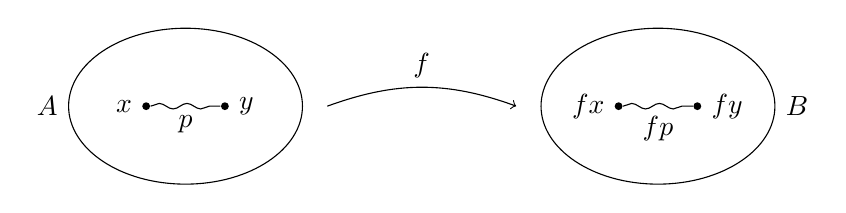
\begin{tikzpicture}
    \def\xshift{6}

    % Base space A
    \node[circle,scale=1.4,draw,inner sep=0.5cm,label=left:{$A$},xscale=1.5] (A) at (0,0) {};
    \node[circle,fill,inner sep=1pt,label=left:{$x$}] (a1) at (-.5,0) {};
    \node[circle,fill,inner sep=1pt,label=right:{$y$}] (a2) at (.5,0) {};
    \draw[decorate,decoration={snake,amplitude=1}] (a1) -- node[auto,swap] {$p$} (a2);

    \draw[->] (1.8,0) to[bend left=20] node[auto] {$f$} (\xshift-1.8,0);

    % Base space B
    \node[circle,scale=1.4,draw,inner sep=0.5cm,label=right:{$B$},xscale=1.5] (B) at (\xshift,0) {};
    \node[circle,fill,inner sep=1pt,label=left:{$\apply{f}{x}$}] (b1) at (\xshift-0.5,0) {};
    \node[circle,fill,inner sep=1pt,label=right:{$\apply{f}{y}$}] (b2) at (\xshift+0.5,0) {};
    \draw[decorate,decoration={snake,amplitude=1}] (b1) -- node[auto,swap] {$\appply{\ap}{f}{p}$} (b2);
    % \draw[decorate,decoration={snake,amplitude=1}] (b1) -- node[auto] {$f(p)$} (b2);
  \end{tikzpicture}
\end{center}

\begin{lemma}[Transport]\label[lemma]{lemma:transport}
  If $A:\universe$, $P:A→\universe$, and $p:\propeq{A}{x}{y}$, then there is a
  function
  \begin{equation*}
    \transport{P}{p} : \apply{P}{x}→\apply{P}{y}
  \end{equation*}
\end{lemma}

In the homotopy model, dependent types $P:A→\universe$ sort of ``lay over'' the
``base space'' $A$. The following is a schematic representation of
$\transportname$ with these metaphors in mind:

\begin{center}
  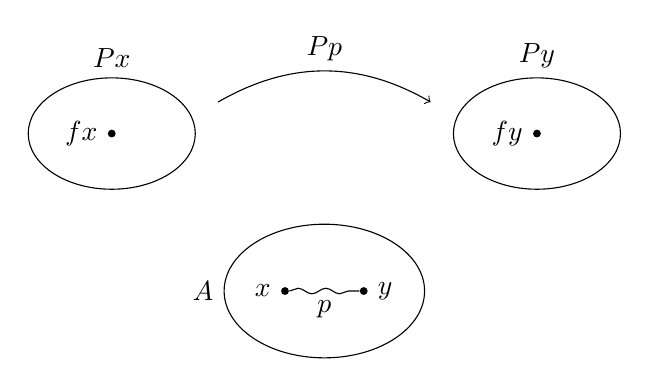
\begin{tikzpicture}
    \def\xshift{2.7}
    \def\yheight{2}

    % P(x)
    \node[circle,draw,inner sep=0.5cm,label=above:{$\apply{P}{x}$},xscale=1.5] (px) at (-\xshift,\yheight) {};
    \node[circle,fill,inner sep=1pt,label=left:{$\apply{f}{x}$}] (b1) at (px) {};

    % P(y)
    \node[circle,draw,inner sep=0.5cm,label=above:{$\apply{P}{y}$},xscale=1.5] (py) at (\xshift,\yheight) {};
    \node[circle,fill,inner sep=1pt,label=left:{$\apply{f}{y}$}] (b1) at (py) {};

    % Base space A
    \node[circle,scale=1.2,draw,inner sep=0.5cm,label=left:{$A$},xscale=1.5] (A) at (0,0) {};
    \node[circle,fill,inner sep=1pt,label=left:{$x$}] (b1) at (-.5,0) {};
    \node[circle,fill,inner sep=1pt,label=right:{$y$}] (b2) at (.5,0) {};
    \draw[decorate,decoration={snake,amplitude=1}] (b1) -- node[auto,swap] {$p$} (b2);

    \draw[->] (-0.5*\xshift,\yheight+0.2*\yheight) to[bend left] node[auto] {$\transpor{P}{p}$} (0.5*\xshift,\yheight+0.2*\yheight);
    % \draw[decorate,decoration={snake,amplitude=1}] (b1) -- node[auto] {$f(p)$} (b2);
  \end{tikzpicture}
\end{center}

Logically, the operation $\transportname$ corresponds to the principle of
``indiscernibility of identicals''. Two equal elements of a type share 
all their properties. For example, if $A\jdeq \N$, $P\jdeq \ttfun{Even}$, 
$z:\apply{\ttfun{Even}}{x}$, and $p:\propeq{}{x}{y}$, then
$\transport{P}{p}{z}$ is a proof that $y$ is even.

\begin{lemma}\label[lemma]{lemma:transport-compose}
	For $f:A\to B$, $P:B\to\universe$, and $p:\propeq{A}{x}{y}$,
  \begin{equation*}
    \propeq{}{
      \transpor{P∘f}{p}
    }{
      \transpor{P}{(\appply{\ap}{f}{p})}
    }
  \end{equation*}
\end{lemma}

Schematically,

\vspace{0.1em}
\begin{tikzpicture}[yscale=.5,xscale=1]
  \def\xshift{3.2}
  \def\yheight{6}

  % P(x)
  \node[circle,draw,inner sep=0.5cm,label=left:{$\apply{P}{(\apply{f}{x})}$}] (px) at (-1.0*\xshift,\yheight) {};
  \node[circle,fill,inner sep=1pt,label=left:{$u$}] (u) at (px) {};

  % P(f(y))
  \node[circle,draw,inner sep=0.6cm,label=above:{$\apply{P}{(\apply{f}{y})}$},yscale=1.5,xscale=3.2] (py) at (1.0*\xshift,\yheight) {};
    \node[circle,fill,inner sep=1pt,label=right:{$\transport{P∘f}{p}{u}$},yshift=0.5] (tpfu) at (0.45*\xshift,1.15*\yheight) {};
  \node[circle,fill,inner sep=1pt,label=right:{$\transport{P}{(\appply{\ap}{f}{p})}{u}$},yshift=0.5] (tpu) at (0.45*\xshift,0.85*\yheight) {};
  \draw[decorate,decoration={snake,amplitude=1}] (tpfu) -- (tpu);

  % P(x) -> P(y)
  \draw[->,shorten >=0.3cm,shorten <=0.3cm, transform canvas={yshift=0.1cm}] (px) to[bend left] node[above] {$\transpor{P\circ f}{p}$} (py) {};
  \draw[->,shorten >=0.3cm,shorten <=0.3cm, transform canvas={yshift=-0.1cm}] (px) to[bend right] node[below] {$\transpor{P}{(\appply{\ap}{f}{p})}$} (py) {};

  % Base space B
  \node[circle,draw,inner sep=0.5cm,label=right:{$B$},xscale=2.2] (B) at (\xshift,0) {};
  \node[circle,fill,inner sep=1pt,label=left:{$\apply{f}{x}$}] (fy) at (\xshift-0.5,0) {};
  \node[circle,fill,inner sep=1pt,label=right:{$\apply{f}{y}$}] (fx) at (\xshift+0.5,0) {};
  \draw[decorate,decoration={snake,amplitude=1}] (fx) -- node[below,swap] {$\appply{\ap}{f}{p}$} (fy);

  % Base space A
  \node[circle,draw,inner sep=0.5cm,label=left:{$A$},xscale=2.2] (A) at (-1.0*\xshift,0) {};
  \node[circle,fill,inner sep=1pt,label=left:{$x$}] (b1) at (-.5-1.0*\xshift,0) {};
  \node[circle,fill,inner sep=1pt,label=right:{$y$}] (b2) at (.5-1.0*\xshift,0) {};
  \draw[decorate,decoration={snake,amplitude=1}] (b1) -- node[auto,swap] {$p$} (b2);

  \draw[->,shorten >=0.1cm,shorten <=0.1cm] (A) to[] node[auto] {$f$} (B) {};
\end{tikzpicture}


\subsection{Σ-types}
\label{subsec:sigma-types}

The \define{dependent pair type}, or Σ-type, generalizes direct products so that
the type of the second projection might depend on the value of the first.
The rules for Σ-types generalize those for direct products in much the same way
Π-types do for function types:
\begin{gatherjot}
  \prftree[r]{}
    {Γ ⊢ A : \universe}
    {Γ,a:A ⊢ B : \universe}
    {Γ ⊢ \sigmatt{a:A}{\apply{B}{a}} : \universe}
  \qquad
  \prftree[r]{}
    {Γ ⊢ a:A}
    {Γ ⊢ b:\apply{B}{a}}
    {Γ ⊢ \dpair{a}{b}:\sigmatt{a:A}{\apply{B}{a}}} \\
  \prftree[r]{}
    {Γ ⊢ {x}:\sigmatt{a:A}{\apply{B}{a}}}
    {Γ ⊢ \appr{1}{x}:A}
  \qquad
  \prftree[r]{}
    {Γ ⊢ {x}:\sigmatt{a:A}{\apply{B}{a}}}
    {Γ ⊢ \appr{2}{x}:A} \\
  \prftree[r]{βΣ\textsubscript{l}}
    {Γ ⊢ b:\apply{B}{a}}
    {Γ ⊢ a:A}
    {Γ ⊢ \appr{1}{\dpair{a}{b}}\jdeq a:A} 
  \qquad
  \prftree[r]{βΣ\textsubscript{r}}
    {Γ ⊢ b:\apply{B}{a}}
    {Γ ⊢ a:A}
    {Γ ⊢ \appr{2}{\dpair{a}{b}}\jdeq b:A}  \\
  \prftree[r]{η}
    {Γ ⊢ f : \pitt{a:A}{\apply{B}{a}}}
    {Γ ⊢ \λ{x}{\apply{f}{x}}\jdeq f:\pitt{a:A}{\apply{B}{a}}}
\end{gatherjot}

Under the types-as-propositions interpretations, Σ-types correspond to
existential quantification: a pair $\dpair{a}{b}:\∑{a:A}{\apply{B}{a}}$
is an element $a:A$ together with a witness or proof term $b$ which demonstrates
that $a$ has the property $B$. This differs significantly from classical notions
of existence. To show that for any $n:\N$, there is a prime greater than $n$ is
to give an \textit{algorithm} for finding said prime.

Additionally, since type theory is \textit{proof-relevant}, one can ``look inside''
an existence proof. Suppose one has $p:\∑{a:A}{\apply{P}{a}}$. Then
$\appr{1}{p}:A$ is exactly whichever $a:A$ was shown to have property $P$!
If one constructs a proof $q$ of another theorem using $p$ and later goes back to
change how $p$ is constructed, it may affect the validity/value of $q$.
This sort of dependence on proof content is not infrequent in classical proofs,
but in that setting is (strictly speaking) an error.

\begin{example}\label[example]{ex:ptd}
	The (universe-polymorphic!) type
  \begin{align*}
    \ttfun{Ptd} : \universe && \ttfun{Ptd}\defeq\∑{A:\universe}{A}
  \end{align*}
  consists of pairs $\dpair{A}{a}$ where $a:A$. We might call this the type of 
  \define{pointed} types.
\end{example}

\subsection{Natural numbers and lists}
\label{subsec:natural-numbers-and-lists}

None of the rules of \UTT{} introduced so far allow for the construction of
infinite types. One principled family of such types are the \textit{inductive}
or \textit{well-founded types}. We call the introduction rules of such types
\define{constructors}. Here, we introduce just two examples: the
natural numbers and lists.

\begin{definition}\label[definition]{def:nat}
	The \define{natural numbers} are the type $\N$ with formation and introduction
  rules
  \begin{align*}
    \prftree[r]{}
      {}
      {Γ ⊢ \N:\universe}
    &&
    \prftree[r]{}
      {}
      {Γ ⊢ 0:\N}
    &&
    \prftree[r]{}
      {Γ ⊢ n:\N}
      {Γ ⊢ \apply{\suc}{n}:\N}
  \end{align*}
  and elimination/computation rules
  \begin{gatherjot}
    \rec_{\N}:\∏{C:\universe} C → (\N→C→C) → \N → C \\
    \appppply{\rec_{\N}}{C}{c}{f}{0} \jdeq c \\
    \appppply{\rec_{\N}}{C}{c}{f}{(\apply{\suc}{n})} \jdeq
    \apply{f}{(\appppply{\rec_{\N}}{C}{c}{f}{n})}
  \end{gatherjot}
  and
  \begin{gatherjot}
    \ind_{\N}:\∏{C:\N→\universe} \apply{C}{0} → \paren{\∏{n:\N}{\apply{C}{n}→\apply{C}{(\apply{\suc}{n})}}} → \∏{n:\N} \apply{C}{n} \\
    \appppply{\ind_{\N}}{C}{c}{f}{0} \jdeq c \\
    \appppply{\ind_{\N}}{C}{c}{f}{(\apply{\suc}{n})} \jdeq
    \apply{f}{(\appppply{\rec_{\N}}{C}{c}{f}{n})}
  \end{gatherjot}
\end{definition}

These rules give some intuition as to why the (dependent) elimination 
rules are called ``recursors'' and ``induction principles'': in the case of
$\N$, they correspond exactly to definition by recursion and the principle of
induction. 

\begin{definition}
  The type of \define{lists} has the following formation and introduction rules:
  \begin{align*}
    \prftree[r]{}
      {Γ ⊢ A:\universei{i}}
      {Γ ⊢ \List{A}:\universei{i}}
    &&
    \prftree[r]{}
      {}
      {Γ ⊢ \nil:\List{A}}
    &&
    \prftree[r]{}
      {Γ ⊢ l:\List{A}}
      {Γ ⊢ a:A}
      {Γ ⊢ \appply{\cons}{a}{l}:\List{A}}
  \end{align*}
  ($\ttfun{List}$ is a \textit{type constructor}, a function
  $\universe→\universe$.) It has the following induction principle:
  \begin{equation*}
    \ind_{\List{A}}:
    \∏{C:\List{A}→\universe}
      {\apply{C}{\nil} →
        \paren{\∏{l:\List{A}}{\∏{a:A}{\apply{C}{l}→\apply{C}{(\appply{\cons}{a}{l})}}}} →
        \∏{l:\List{A}} \apply{C}{l}}
  \end{equation*}
  (With appropriate β-rules, not included here.)
\end{definition}

The introduction rule $\cons$ takes an element of $A$ and prepends it onto the
front of the list. This inductive presentation of lists owes much to the
\software{Lisp} programming language.

\section{h-levels}
\label{sec:h-levels}

One of the central organizational innovations of \UTT{} is a focus on h-levels. 
While universes (roughly) stratify types by their ``size'', h-levels stratify
them by the non-triviality of their nested equality types.

\begin{figure}[ht]
  \centering
  \begin{tikzpicture}
    \draw[step=1.0,black,thin] (0.0,0.0) grid (6,5);
    \draw[->, black, thick] (0.0,0.0) -- (0,5.5) node[above] {\text{size}};
    \draw[->, black, thick] (0.0,0.0) -- (6.5,0) node[right] {\text{hlevel}};

    % universe levels
    \node[] at (-0.5, 1.0) {$\universei{0}$};
    \node[] at (-0.5, 2.0) {$\universei{1}$};
    \node[] at (-0.5, 3.0) {$\universei{2}$};
    \node[] at (-0.5, 4.0) {$\vdots$};
    \node[] at (-0.5, 5.0) {$\universei{n}$};

    % hlevels
    \node[rotate=270, anchor=west] at (1.0, -0.5) {contractible};
    \node[rotate=270, anchor=west] at (2.0, -0.5) {proposition};
    \node[rotate=270, anchor=west] at (3.0, -0.5) {set};
    \node[rotate=270, anchor=west] at (4.0, -0.5) {groupoid};
    \node[rotate=270, anchor=west] at (5.0, -0.5) {$\cdots$};
    \node[rotate=270, anchor=west] at (6.0, -0.5) {$n$-groupoid};

    % types
    \node[anchor=west] at (1.0, 1.3) {$\unittype$};
    \node[scale=3] at (1.0, 0.9) {$\cdot$};

    \node[anchor=west] at (3.0, 1.3) {$\N$};
    \node[scale=3] at (3.0, 0.9) {$\cdot$};

    \node[anchor=west] at (2.0, 3.5) {$\∏{X:\universei{1}}\apply{\isProp}{X}$};
    \node[scale=3] at (2.0, 2.9) {$\cdot$};
    
  \end{tikzpicture}
  \caption{\label{fig:awodey} Awodey's two axes: size (universe level)
    and complexity (h-level) \cite{awodey-proposition-homotopy-type}.}
\end{figure}

\begin{definition}\label[definition]{def:mere-proposition}
  A type $X:\universe$ is a \define{mere proposition}, a \define{proposition},
  an \define{hprop}, or is \define{of h-level $1$}\footnote{More on this soon.}
  if all of its elements are propositionally equal,
  \begin{equation*}
    \apply{\isProp}{X} \defeq \pit{x,y:X}x=y
  \end{equation*}
\end{definition}

Mere propositions act significantly more like propositions in \FOL{},
in that they are \textit{proof-irrelevant}: a proof of a proposition contains no
other information than that the proposition is in fact inhabited (any two such
proofs are equal). The UIP principle can be rephrased as ``identity types are
propositions''.

\begin{definition}\label[definition]{def:contr}
  A type $X:\universe$ is \define{contractible} or is \define{of h-level $0$}
  if it is a mere proposition and is inhabited, that is
  \begin{equation*}
    \apply{\isContr}{X} \defeq \sigmat{x:X}{\pit{y:X}x=y}
  \end{equation*}
  The first projection is the \define{center} of $X$.
\end{definition}

\begin{lemma}\label[lemma]{lemma:unit-contr}
	The unit type $\unittype$ is contractible.
\end{lemma}
\begin{proof}
	Use the dependent elimination rule for $\unittype$ with the family
  \begin{equation*}
    C\defeq \λ{x}{\propeq{}{\unitelem}{x}}.
  \end{equation*}
\end{proof}

Despite \cref{rmk:uip}, we can prove the following:

\begin{lemma}
	For any $A:\universe$ and $a:A$, the types $\∑{x:A}{\propeq{}{x}{a}}$
  and $\∑{x:A}{\propeq{}{a}{x}}$ are contractible.
\end{lemma}

There are certain types for which UIP does hold:

\begin{definition}\label[definition]{def:sets}
  A type is a \define{set} or \define{hset} if its identity types are
  propositions. That is, for $A:\universe$
  \begin{equation*}
    \apply{\isSet}{A}\defeq \∏{x,y:A}{\apply{\isProp}{(\propeq{}{x}{y})}}
  \end{equation*}
\end{definition}

While the metaphor can be made more precise in a variety of ways, suffice to say
that when working in type theory it seems that in practice almost all intuitions
and arguments about sets in carry over to sets in \UTT{} (modulo constructivity).

\begin{definition}
	A type $A:\universe$ is \define{of h-level $n$} if its identity types are of
  h-level $n-1$. That is,
  \begin{alignat*}{3}
    &\hlevel &&: \N → \universe → \universe \\
    &\appply{\hlevel}{0}{A} &&\defeq \apply{\isContr}{A} \\
    &\appply{\hlevel}{(\apply{\suc}{n})}{A} &&\defeq
    \∏{x,y:A}{\appply{\hlevel}{n}{(\propeq{}{x}{y}})}
  \end{alignat*}
  (Note that we implicitly use the elimination rules for $\N$ when defining
  functions via \textit{pattern matching}.)\footnote{It may be useful to review
  contractible types, propositions, and sets to ensure that they do indeed follow
  this pattern.}
\end{definition}

\begin{lemma}\label[lemma]{lemma:impred}
  If $X:\universe$, $Y:X→\universe$, and each $\apply{Y}{x}$ is of h-level $n$,
  then $\∏{x:X}{\apply{Y}{x}}$ is of h-level $n$.
\end{lemma}

It is worth mentioning that (with additional axioms) given any type $X$, there
is a formalism in \HoTT{} for constructing its $n$-truncation $∥X∥_n$, which
is guaranteed to be of h-level $n$ or lower.

\section{Univalence}
\label{sec:univalence}

\subsection{Weak equivalences}
\label{subsec:weak-equivalences}

Weak equivalences are another innovation of the homotopy type theory community.
They are necessary to state the univalence axiom (and are generally useful!).
There are several equivalent (and individually enlightening) ways to
characterize such equivalences, these require a few preliminary definitions.

\begin{definition}\label[definition]{def:fiber}
	Given a function $f:A→B$ and point $b:B$, the \define{fiber of $f$ above $b$}
  is the type
  \begin{equation*}
    \apply{\ttfun{fiber}_f}{b}\defeq\∑{a:A}{\propeq{}{\apply{f}{a}}{b}}
  \end{equation*}
\end{definition}

\begin{definition}
	Given dependent functions $f,g:\∏{a:A}{\apply{B}{a}}$, a \define{homotopy}
  between them is an inhabitant of
  \begin{equation*}
    f\sim g\defeq \∏{a:A}{\propeq{}{\apply{f}{a}}{\apply{g}{a}}}
  \end{equation*}
\end{definition}

\begin{definition}\label[definition]{def:weq}
  A function $f:A→B$ is a weak equivalence if any of the following
  equivalent\footnote{For proofs that these characterizations are mutually
    equivalent, see \cite{book}. The type of equivalence meant in the phrase
    ``equivalent definitions'' can be understood as any of the ones being defined.}
  conditions hold:
  \begin{itemize}
    \itemsep0em
    \item the fibers of $f$ are contractible,
      $\∏{b:B}{\apply{\isContr}{(\apply{\ttfun{fiber}_f}{b}})}$,
    \item there are functions $g,h:B→A$ such that their compositions
      with $f$ are the appropriate identities:
      \begin{equation*}
        \paren{\∑{g:B→A}{f∘g\sim \id_B}}×\paren{\∑{h:B→A}{h∘f\sim\id_A}},
      \end{equation*}
      or
    \item there is a function $g:B→A$ with homotopies $η:g∘f\sim\id_A$,
      $ε:f∘g\sim\id_B$, and
      $τ:\∏{a:A}{\propeq{}{\apply{f}{(\apply{η}{a})}}{\apply{ε}{(\apply{f}{a}})}}$.
  \end{itemize}
  We abusively denote the type of any of these conditions by
  $\apply{\isEquiv}{f}$. When $f:A→B$ is an equivalence, we write
  $f:\weq{A}{B}$, and may write $\weq{A}{B}$ to indicate that such an $f$
  exists.
\end{definition}

\begin{lemma}\label[lemma]{lemma:isequiv-prop}
	\
  \begin{enumerate}
    \itemsep0em
    \item The property of being a weak equivalence is a proposition.
    \item The composition of weak equivalences is again a weak equivalence.
    \item The relation $\weqsign$ is an equivalence relation on $\universe$.
  \end{enumerate}
\end{lemma}

\begin{remark}\label[remark]{rmk:logeq}
  Under the propositions/types correspondence, we might define
  types $A,B:\universe$ to be \textit{logically equivalent} if
  \begin{equation*}
    (A→B)×(B→A)
  \end{equation*}
  (compare to \cref{rmk:n-true}). As can be read off the various definitions of
  weak equivalences, this is a strictly weaker condition.
  Tellingly, logical equivalence and weak equivalence coincide for propositions:
  if $A$ and $B$ are propositions then
  \begin{equation*}
    \weq{(\weq{A}{B})}{\paren{(A→B)×(B→A)}}
  \end{equation*}
\end{remark}

\begin{notation}\label[notation]{notation:weq-coerce}
  We may treat a weak equivalence as if it were a function and apply it to an
  argument. This amounts to implicitly applying $\pr{1}$.
\end{notation}

\begin{lemma}\label[lemma]{lemma:contr-weq-unit}
	Any contractible type is weakly equivalent to $\unittype$.
\end{lemma}
\begin{proof}
	Suppose $X:\universe$ is contractible with center $x$. Define $f:X→\unittype$
  as $\λ{x}{\unitelem}$ and $g:\unittype→X$ as $\λ{u}{x}$. Then by hypothesis on
  $X$, the induction principle for $\unittype$\TODO{reference}, and function
  extensionality (\cref{thm:funext}), the composites are the appropriate
  identities.
\end{proof}

\begin{corollary}\label[corollary]{cor:weq-contr}
	If $w:\weq{A}{B}$ and $B$ is contractible, so is $A$.
\end{corollary}
\begin{proof}
  By \cref{lemma:contr-weq-unit}, $\weq{B}{\unittype}$. Composing with this
  equivalence gives one $\weq{A}{\unittype}$ (\cref{lemma:isequiv-prop}).
\end{proof}

\begin{lemma}\label[lemma]{lemma:weq-eq}
  If $A,B:\universe$, $w:\weq{A}{B}$, and $x,y:A$ then
  \begin{equation*}
    \weq{(\propeq{B}{\apply{w}{x}}{\apply{w}{y}})}{(\propeq{A}{x}{y})}
  \end{equation*}
\end{lemma}
\begin{proof}[Proof sketch]
  If $p:\propeq{A}{x}{y}$, then
  $\appply{\ap}{w}{p}:\propeq{B}{\apply{w}{x}}{\apply{w}{y}}$. Conversely,
  suppose $\propeq{B}{\apply{w}{x}}{\apply{w}{y}}$.
  Then $x$ and $y$ are both in the fiber above $\apply{w}{x}$,
  and since the fibers of a weak equivalence are contractible, $x=y$.
\end{proof}

\begin{lemma}\label[lemma]{lemma:weqfibtototal}
  For any $A:\universe$ and $P,Q:A→\universe$,
  if $\weq{\apply{P}{a}}{\apply{Q}{a}}$ for every $a:A$, then
  \begin{align*}
    \weq{\∏{a:A}{\apply{P}{a}}}{\∏{a:A}{\apply{Q}{a}}}
    &&\text{and}&&
    \weq{\∑{a:A}{\apply{P}{a}}}{\∑{a:A}{\apply{Q}{a}}}
  \end{align*}
\end{lemma}

\subsection{Characterization of paths}
\label{subsec:characterization-of-paths}

A rich family of applications for weak equivalences comes from characterizing
path spaces, that is, saying what counts as an equality between the elements of
a type. For instance, the following restates the η-rule for the product type as
a weak equivalence:

\begin{lemma}\label[lemma]{lemma:paths-dirprod-weq}
  For any $A,B:\universe$, $a:A$, $b:B$, and $x:A×B$,
  \begin{equation*}
    \weq{\big((\propeq{A}{\appr1{x}}{a})×(\propeq{B}{\appr1{x}}{b})\big)}
        {\big(\propeq{}{x}{(a,b)}\big)}
  \end{equation*}
  That is, pairs are equal just when their components (projections) are.
\end{lemma}

The above lemma cannot be generalized as-is to Σ-types, whose second projections
aren't of the same type. However, we have the following (incredibly useful)
lemma, inspired by the homotopy interpretation:

\begin{lemma}\label[lemma]{lemma:path-sigma}
	If $x,y:\∑{a:A}{\apply{B}{a}}$, then
  \begin{equation*}
    \weq{
      (\propeq{}{x}{y})
    }{
      \∑{
        p:\propeq{}{\appr{1}{x}}{\appr{1}{y}}
      }{
        \propeq{}{
          \transport{B}{p}{(\appr{2}{x})}
        }{
          \appr{2}{y}
        }
      }
    }.
  \end{equation*}
\end{lemma}

Schematically,

\begin{center}
  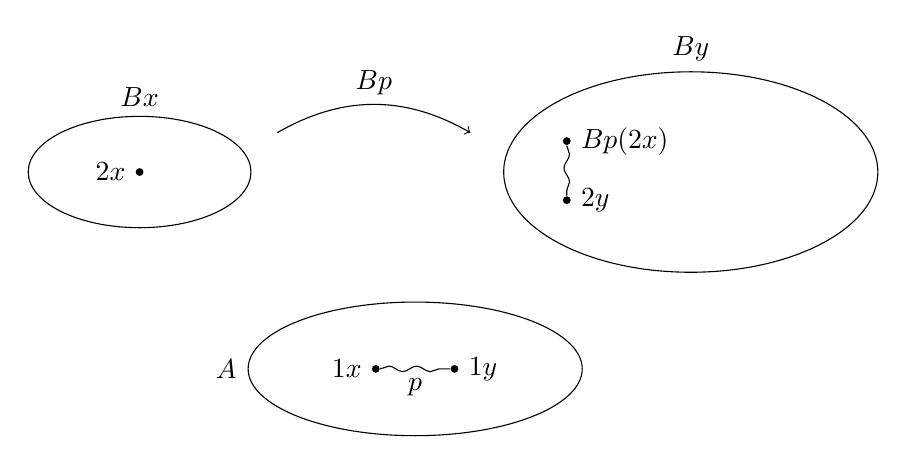
\begin{tikzpicture}
    \def\xshift{3.5}
    \def\yheight{2.5}

    % B(x)
    \node[circle,draw,inner sep=0.5cm,label=above:{$\apply{B}{x}$},xscale=2.0] (px) at (-\xshift,\yheight) {};
    \node[circle,fill,inner sep=1pt,label=left:{$\appr{2}{x}$}] (b1) at (px) {};

    % B(y)
    % \node[circle,draw,inner sep=0.5cm,label=above:{$\apply{B}{y}$},scale=2] (py) at (\xshift,\yheight) {};
    % \node[circle,fill,inner sep=1pt,label=left:{$\appr{2}{y}$}] (b1) at (py) {};

    % B(y)
    \node[circle,draw,inner sep=0.6cm,label=above:{$\apply{B}{y}$},yscale=1.5,xscale=2.8] (py) at (1.0*\xshift,\yheight) {};
    \node[circle,fill,inner sep=1pt,label=right:{$\transport{B}{p}{(\appr{2}{x})}$},yshift=0.5] (tpfu) at (0.55*\xshift,1.15*\yheight) {};
    \node[circle,fill,inner sep=1pt,label=right:{$\appr{2}{y}$},yshift=0.5] (tpu) at (0.55*\xshift,0.85*\yheight) {};
    \draw[decorate,decoration={snake,amplitude=1}] (tpfu) -- (tpu);

    % Base space A
    \node[circle,scale=1.2,draw,inner sep=0.5cm,label=left:{$A$},xscale=2.5] (A) at (0,0) {};
    \node[circle,fill,inner sep=1pt,label=left:{$\appr{1}{x}$}] (b1) at (-.5,0) {};
    \node[circle,fill,inner sep=1pt,label=right:{$\appr{1}{y}$}] (b2) at (.5,0) {};
    \draw[decorate,decoration={snake,amplitude=1}] (b1) -- node[auto,swap] {$p$} (b2);

    \draw[->] (-0.5*\xshift,\yheight+0.2*\yheight) to[bend left] node[auto] {$\transpor{B}{p}$} (0.2*\xshift,\yheight+0.2*\yheight);
  \end{tikzpicture}
\end{center}

\subsection{The univalence axiom}
\label{subsec:the-univalence-axiom}

The univalence axiom characterizes paths in $\universe$. It states that such
paths $\propeq{\universe}{A}{B}$ are exactly the weak equivalences $\weq{A}{B}$.

\begin{definition}\label[definition]{def:ua}
  There is a canonical function
  \begin{equation*}
    \ttfun{idtoweq} : \∏{A,B:\universe}{\propeq{}{A}{B}→\weq{A}{B}}
  \end{equation*}
  defined by path induction and the identity equivalence (the reflexivity of
  $\weqsign$). The \define{univalence axiom} states that $\ttfun{idtoweq}$ is an
  equivalence.\footnote{Note that there are several ways one might define
    $\ttfun{idtoweq}$. \cite{book} uses an alternative definition, we follow
    the \UniMath{} library.} In particular, it has an inverse
  \begin{equation*}
    \ua : \∏{A,B:\universe}{\weq{A}{B}→\propeq{}{A}{B}}
  \end{equation*}
  The axiom may be more concisely yet less precisely stated:
  \begin{equation*}
    \weq{(\propeq{\universe}{A}{B})}{(\weq{A}{B})}
  \end{equation*}
  It has the following computation rule:\footnote{Which is a
  \textit{propositional} equality. Recall that it is incoherent to postulate
  judgmental equalities, which are not part of the language of \UTT{}. 
  There are efforts to construct so-called ``cubical'' type theories in which
  univalence is not an axiom, but can be derived. Generally, this β-rule
  is judgmental in such systems.}
  \begin{equation*}
    \transport{\id_\universe}{(\apply{\ua}{p})}{x} = \apply{p}{x}.
  \end{equation*}
\end{definition}

Intensional equality in type theory has bountiful benefits (decidability of type
checking and interesting model theory, to name two). However, a particular
extensional principle called \textit{function extensionality} seems essential to
standard reasoning. Luckily, it follows from the univalence axiom:

\begin{theorem}\label[theorem]{thm:funext}
  There is a term
  \begin{equation*}\label{eq:funext}
    \ttfun{eqtohomot}:\∏{A,B\:\universe}{\∏{f,g:A→B}{\propeq{}{f}{g}→\homot{f}{g}}}
  \end{equation*}
  defined by identity elimination. Under the hypothesis of the univalence axiom,
  this function is an equivalence. In particular, it has an inverse
  \begin{equation*}\label{eq:funext}
    \funext:\∏{A,B\:\universe}{\∏{f,g:A→B}{(\homot{f}{g})\to \propeq{}{f}{g}}}
  \end{equation*}
\end{theorem}

Function extensionality can be considered a characterization of paths for Π-types.

As a simple example of the use of univalence, we can generalize
\cref{lemma:contr-weq}.

\begin{theorem}
	Weak equivalences preserve h-levels.
\end{theorem}
\begin{proof}
  Let $A,B:\universe$, $n:\N$, $w:\weq{A}{B}$, and $i:\appply{\hlevel}{n}{A}$.
	Univalence provides an equality $\apply{\ua}{w}:\propeq{\universe}{A}{B}$. 
  Then
  \begin{equation*}
    \transport{\apply{\hlevel}{n}}{(\apply{\ua}{w})}{i} : \appply{\hlevel}{n}{B}
  \end{equation*}
\end{proof}

This argument isn't actually specific to contractibility; using univalence any
proposition of the form ``If $\weq{A}{B}$ and $\apply{P}{A}$, then $\apply{P}{B}$''
is trivially true. Briefly, everything respects weak equivalences.

\begin{theorem}
	UIP is inconsistent with the univalence axiom. In particular, there are some
  types that are not sets.
\end{theorem}
\begin{proof}[Proof sketch]
  If UIP holds, then every type is a set. Thus, it suffices to show that $\universe$
  is not a set, i.e.\ that there is a type $A:\universe$ and some equality
  $\propeq{}{A}{A}$ which is not equal to $\refl{A}$. Use $A\defeq\booltype$.
  There are two weak equivalences $\weq{A}{A}$, $\id_A$ and the one that flips
  $\btrue$ and $\bfalse$. It can be shown that if these equivalences gave rise
  to the same equality $\propeq{}{A}{A}$ by univalence, then it would have to be
  the case that $\propeq{}{\btrue}{\bfalse}$, which can shown to be false.
\end{proof}

\end{document}
